\section{EBSD}


\subsection*{Importing EBSD Data}

\begin{frame}[fragile]
  \frametitle{Importing EBSD Data}

  File formats supported by \MTEX

  \medskip

  \begin{columns}
    \begin{column}{5cm}
      \begin{tabular}{ll}
        Fileextension & Format \\
        \toprule
        .ang& TLS \\
        .ctf& HKL \\
        .csv& Oxford
      \end{tabular}

    \end{column}
    \begin{column}{5cm}
      \begin{tabular}{ll}
        Fileextension & Format \\
        \toprule
        .sor& LaboTEX \\
        .txt & generic\\
        .xls & generic
      \end{tabular}
    \end{column}
  \end{columns}

  \pause

  \bigskip

  Script generated by the import wizard

\begin{lstlisting}
CS = { symmetry('m-3m','mineral','Fe'), ...
       symmetry('m-3m','mineral','Mg') }
SS = symmetry('triclinic');
\end{lstlisting}

\begin{lstlisting}
fname = { [ pathto '85_829grad_07_09_06.txt']};
\end{lstlisting}

\begin{actionenv}<1-| alert@1->
\begin{lstlisting}
 ebsd = loadEBSD(fname,CS,SS,'ignorePhase',0,...
 'ColumnNames',{'x' 'y' 'phi1' 'Phi' 'phi2' 'MAD'});
\end{lstlisting}
\end{actionenv}

\end{frame}


\subsection*{Visualization}

\begin{frame}[fragile]
  \frametitle{Visualize EBSD Data in \MTEX}

  \begin{columns}
    \begin{column}{8.5cm}

Scatter plots in Rodrigues space or axis angle space

\begin{lstlisting}
scatter(ebsd)
\end{lstlisting}

\pause

Scatter plots in pole figures, inverse pole figures, or ODF sections


\begin{onlyenv}<1,3- |handout:1>
\begin{lstlisting}
		plotpdf(ebsd,[Miller(0,0,1),...])
		plotipdf(ebsd,vector3d(1,0,0))
		plotodf(ebsd)
\end{lstlisting}
\end{onlyenv}

\begin{onlyenv}<2 |handout:0>
\begin{lstlisting}
		/+plotpdf(ebsd,[Miller(0,0,1),...])+/
		plotipdf(ebsd,vector3d(1,0,0))
		plotodf(ebsd)
\end{lstlisting}
\end{onlyenv}

\pause

Spatial plots of EBSD data

\begin{onlyenv}<1-2|handout:0>
\begin{lstlisting}
plot(ebsd)
plot(ebsd,'colorcoding','ipdf')
plot(ebsd,'property','phase')
plot(ebsd,'property','mad')
\end{lstlisting}
\end{onlyenv}

\begin{onlyenv}<3 |handout:1>
\begin{lstlisting}
/+plot(ebsd)+/
/+plot(ebsd,'colorcoding','ipdf')+/
plot(ebsd,'property','phase')
plot(ebsd,'property','mad')
\end{lstlisting}
\end{onlyenv}

\begin{onlyenv}<4 |handout:0>
\begin{lstlisting}
plot(ebsd)
plot(ebsd,'colorcoding','ipdf')
/+plot(ebsd,'property','phase')+/
plot(ebsd,'property','mad')
\end{lstlisting}
\end{onlyenv}

\begin{onlyenv}<5 |handout:0>
\begin{lstlisting}
plot(ebsd)
plot(ebsd,'colorcoding','ipdf')
plot(ebsd,'property','phase')
/+plot(ebsd,'property','mad')+/
\end{lstlisting}
\end{onlyenv}

      Color-Codings: ipdf, hkl, bunge, angle

    \end{column}

    \begin{column}{3.5cm}
      \only<1 |handout:0>{%
      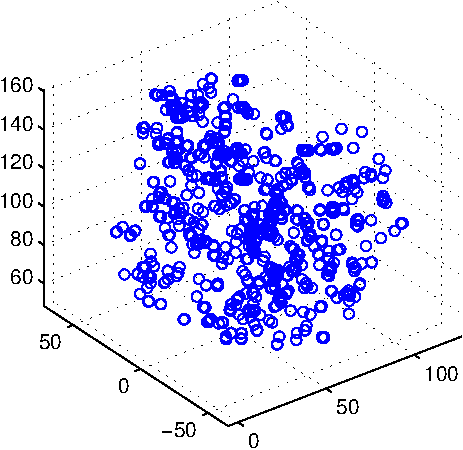
\includegraphics[width=3.5cm]{pic/ebsdscatter}%
      }%
      \only<2|handout:0>{%
      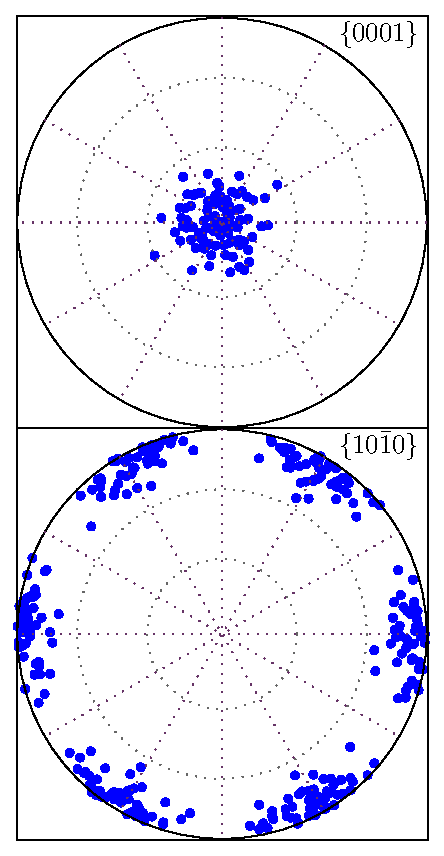
\includegraphics[width=3.2cm]{pic/EBSDpdf}%
      }%
      \only<3|handout:1>{%
      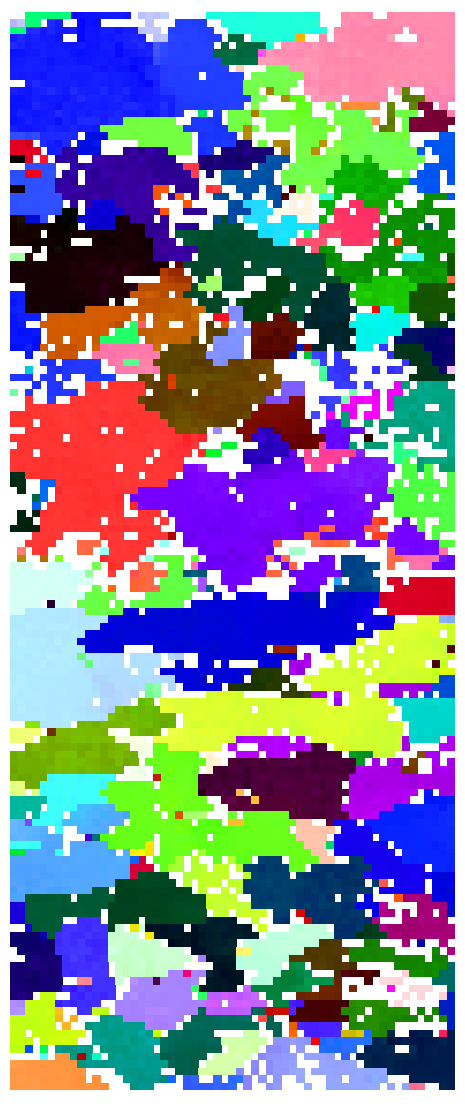
\includegraphics[height=7.5cm]{pic/ebsdsmall}%
      }%
      \only<4|handout:0>{%
      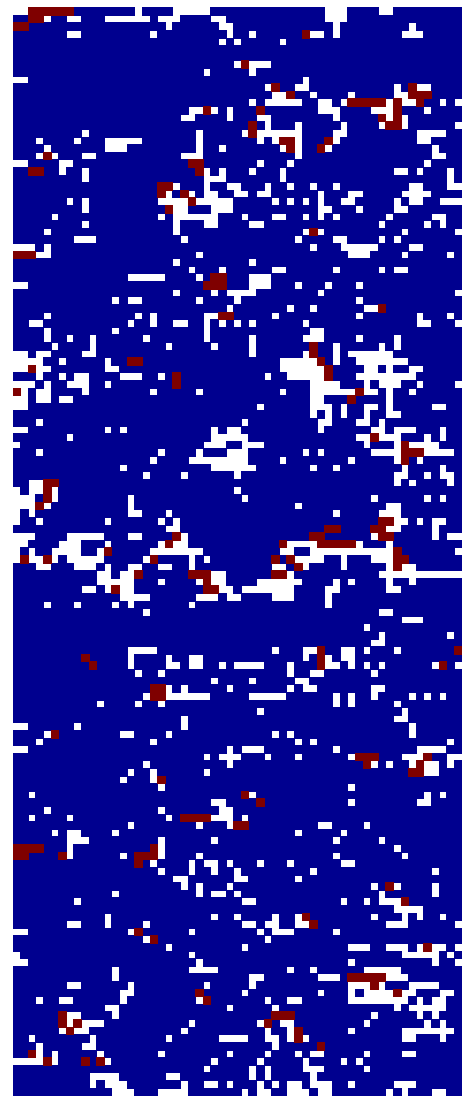
\includegraphics[height=7.5cm]{pic/ebsdphase}%
      }%
      \only<5|handout:0>{%
      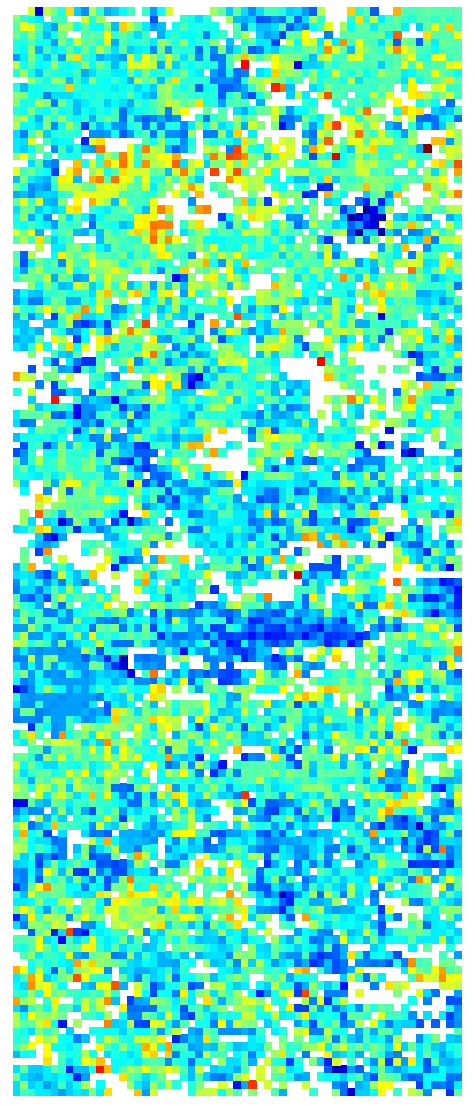
\includegraphics[height=7.5cm]{pic/ebsdmad}%
      }%
    \end{column}
  \end{columns}
\end{frame}

\subsection*{Grains Analysis}

\begin{frame}[fragile]
  \frametitle{Grain Analysis with \mtex}

  \begin{columns}
    \begin{column}{8.5cm}

      \medskip

      Grain Detection

\begin{lstlisting}
[grains ebsd] = calcGrains(ebsd,...
    'angle',10*degree)
\end{lstlisting}

% \begin{tabular}{ll}
%   Option & Value \\
%   \toprule
%   angle &  threshold angle\\
%   distance &  max distance\\
%   augmentation & bounding box\\
%   unitcell &  use a unitcell
% \end{tabular}

\medskip

Plot grain boundaries:
\begin{lstlisting}
hold on
plotboundary(grains,/+<options>+/)
\end{lstlisting}

\begin{tabular}{ll}
  Option & Value \\
  \toprule
  color & red, blue, black, green\\
  linewidth & number of points\\
  property & phase, missorientation\\
\end{tabular}

\end{column}
    \begin{column}{3.5cm}
      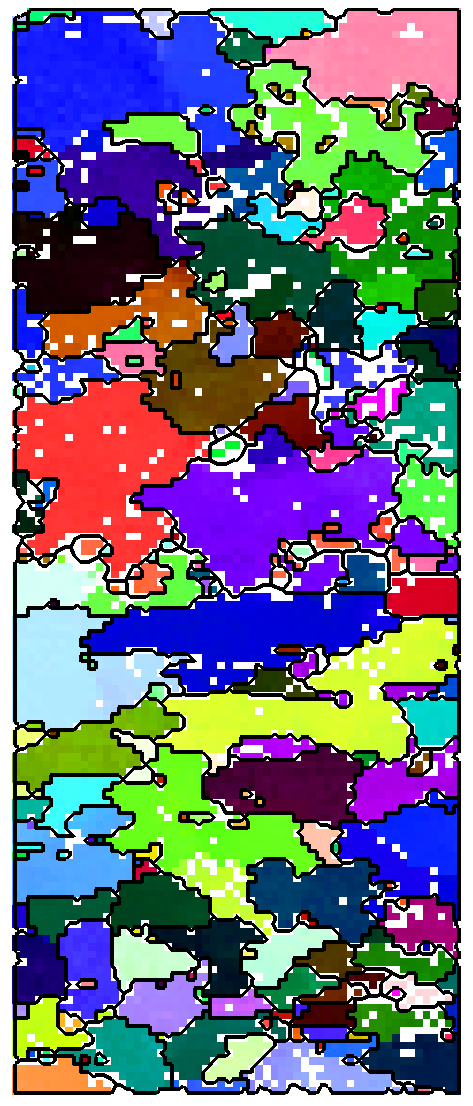
\includegraphics[height=7.5cm]{pic/ebsdgrains}
    \end{column}
  \end{columns}

\end{frame}


\subsection*{Grain Properties}


\begin{frame}[fragile]
  \frametitle{Grain Properties}

  \begin{columns}
    \begin{column}{8.5cm}

      Plotting grains
      \begin{onlyenv}<1 |handout:1>
\begin{lstlisting}
plot(grains,'property','orientation')
\end{lstlisting}
      \end{onlyenv}

      \begin{onlyenv}<2- |handout:0>
\begin{lstlisting}
plot(grains,'property',/+'phase'+/)
\end{lstlisting}
      \end{onlyenv}

      \pause
      \pause

\bigskip

      Access grain properties
\begin{lstlisting}
phase  = get(grains,'phase')
grain1 = grains(phase == 1)
ori    = get(grain1,'orientation')
\end{lstlisting}

\pause

\bigskip

Access individual grains
\begin{lstlisting}
plot(grain(200))
\end{lstlisting}

\pause
\bigskip

smooth grain boundaries
\begin{lstlisting}
grains = smooth(grains,2,'S')
\end{lstlisting}



% Interconnection with EBSD Data
% \begin{lstlisting}
% gS = grainSize(grains)
% largeGrains = grains(gs>10)
% large_ebsd = link(largeGrains,ebsd)
% \end{lstlisting}

    \end{column}
    \begin{column}{3.5cm}
      \only<1|handout:1>{%
      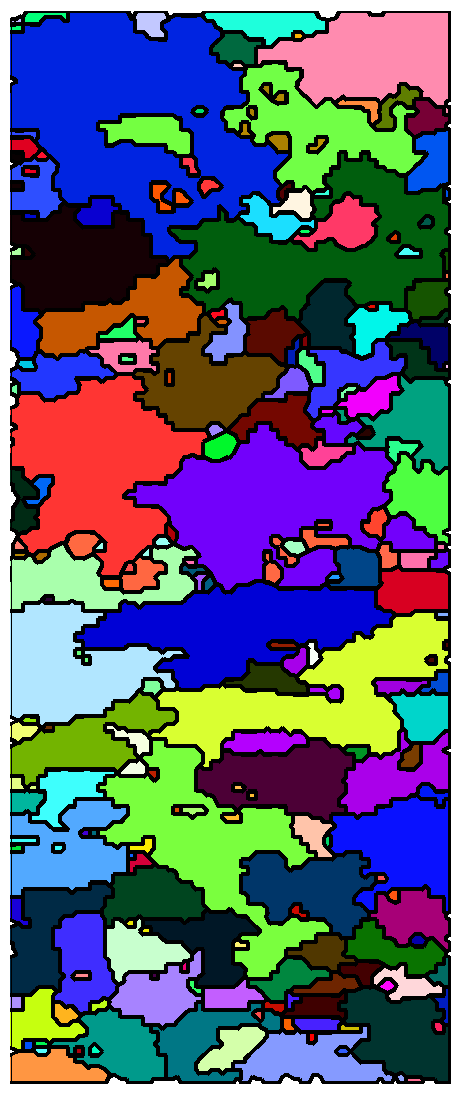
\includegraphics[height=7.5cm]{pic/ebsdgrainorientation}%
      }%
      \only<2-3|handout:0>{%
      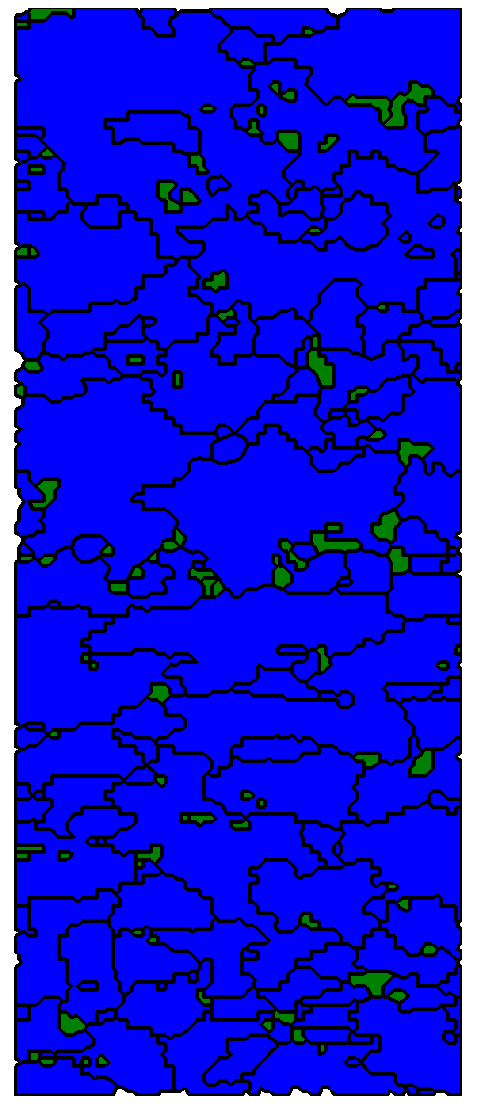
\includegraphics[height=7.5cm]{pic/ebsdgrainsphase}%
      }%
      \only<4|handout:0>{%
      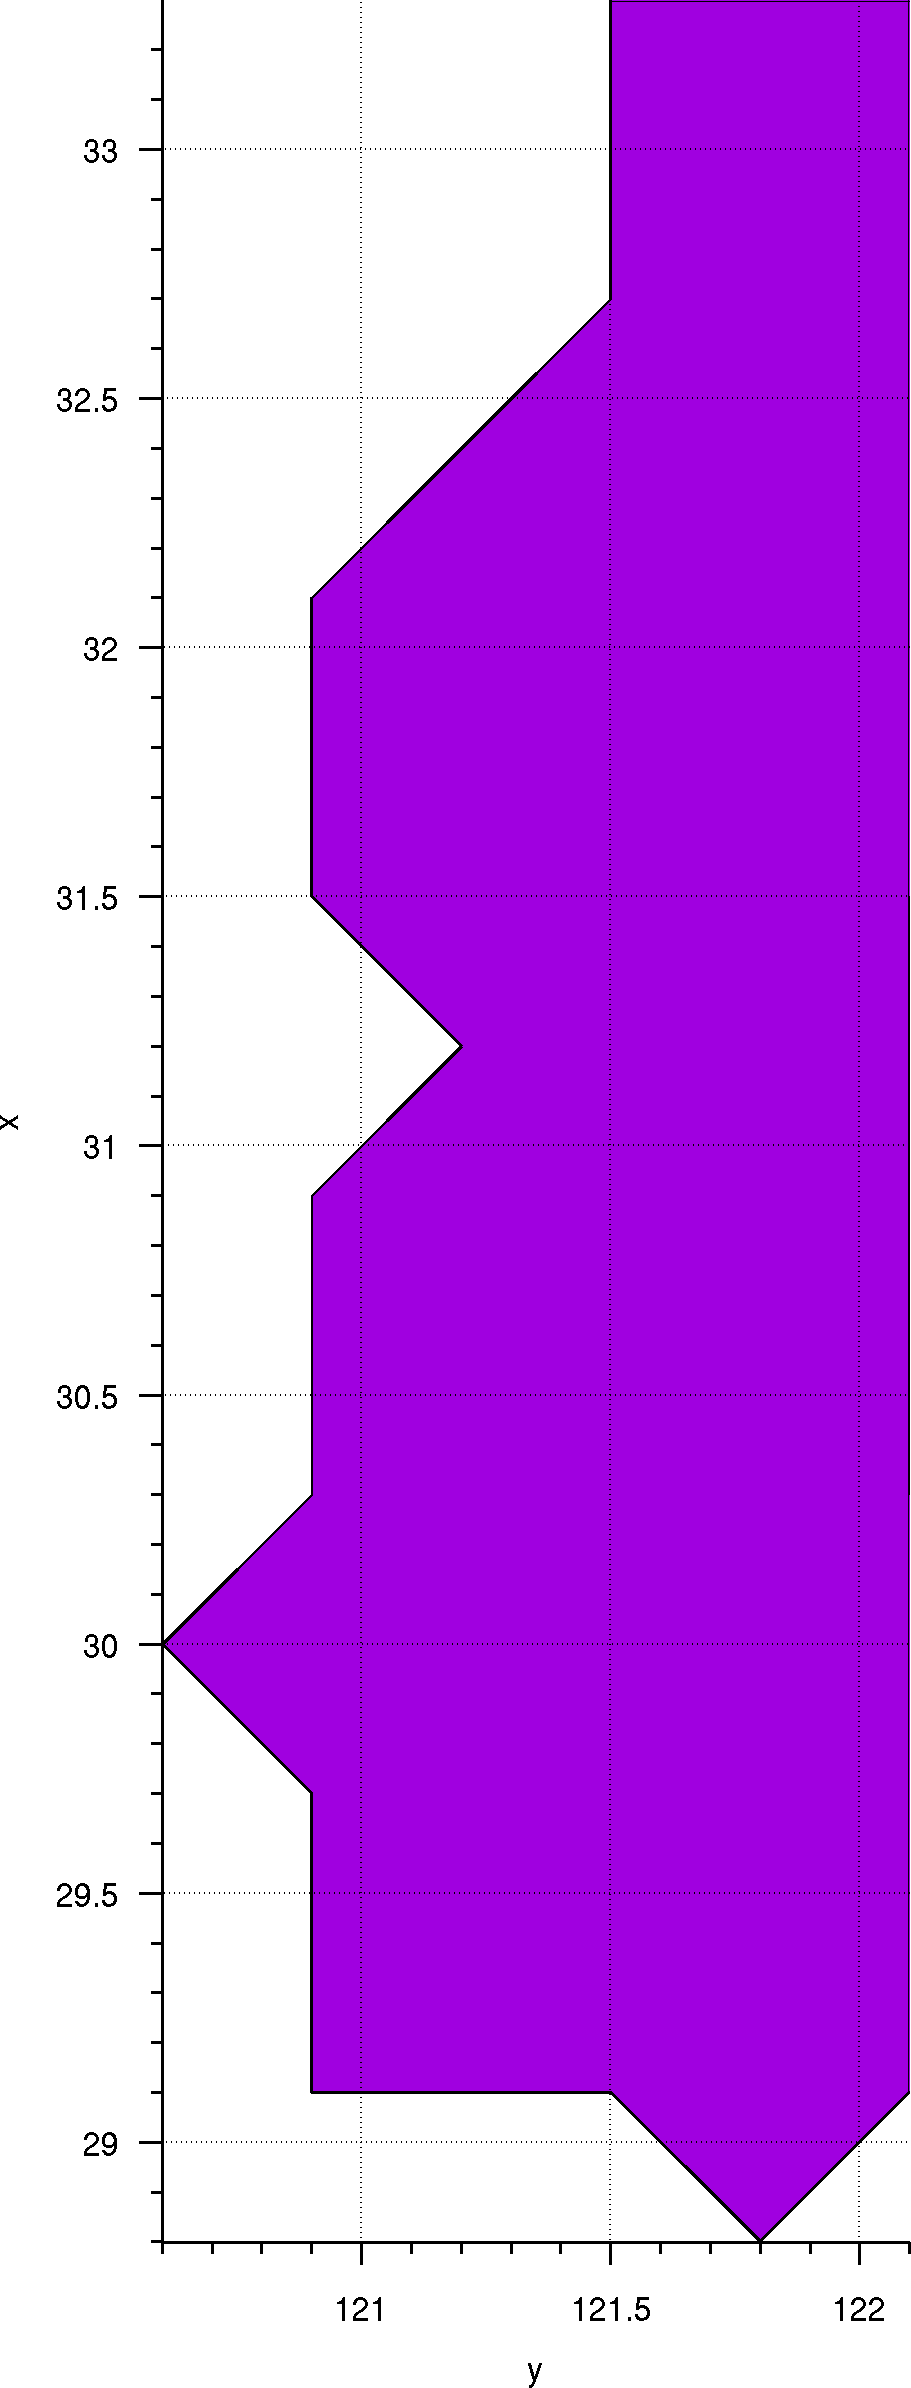
\includegraphics[height=8cm]{pic/grain.png}%
      }%
      \only<5|handout:0>{%
      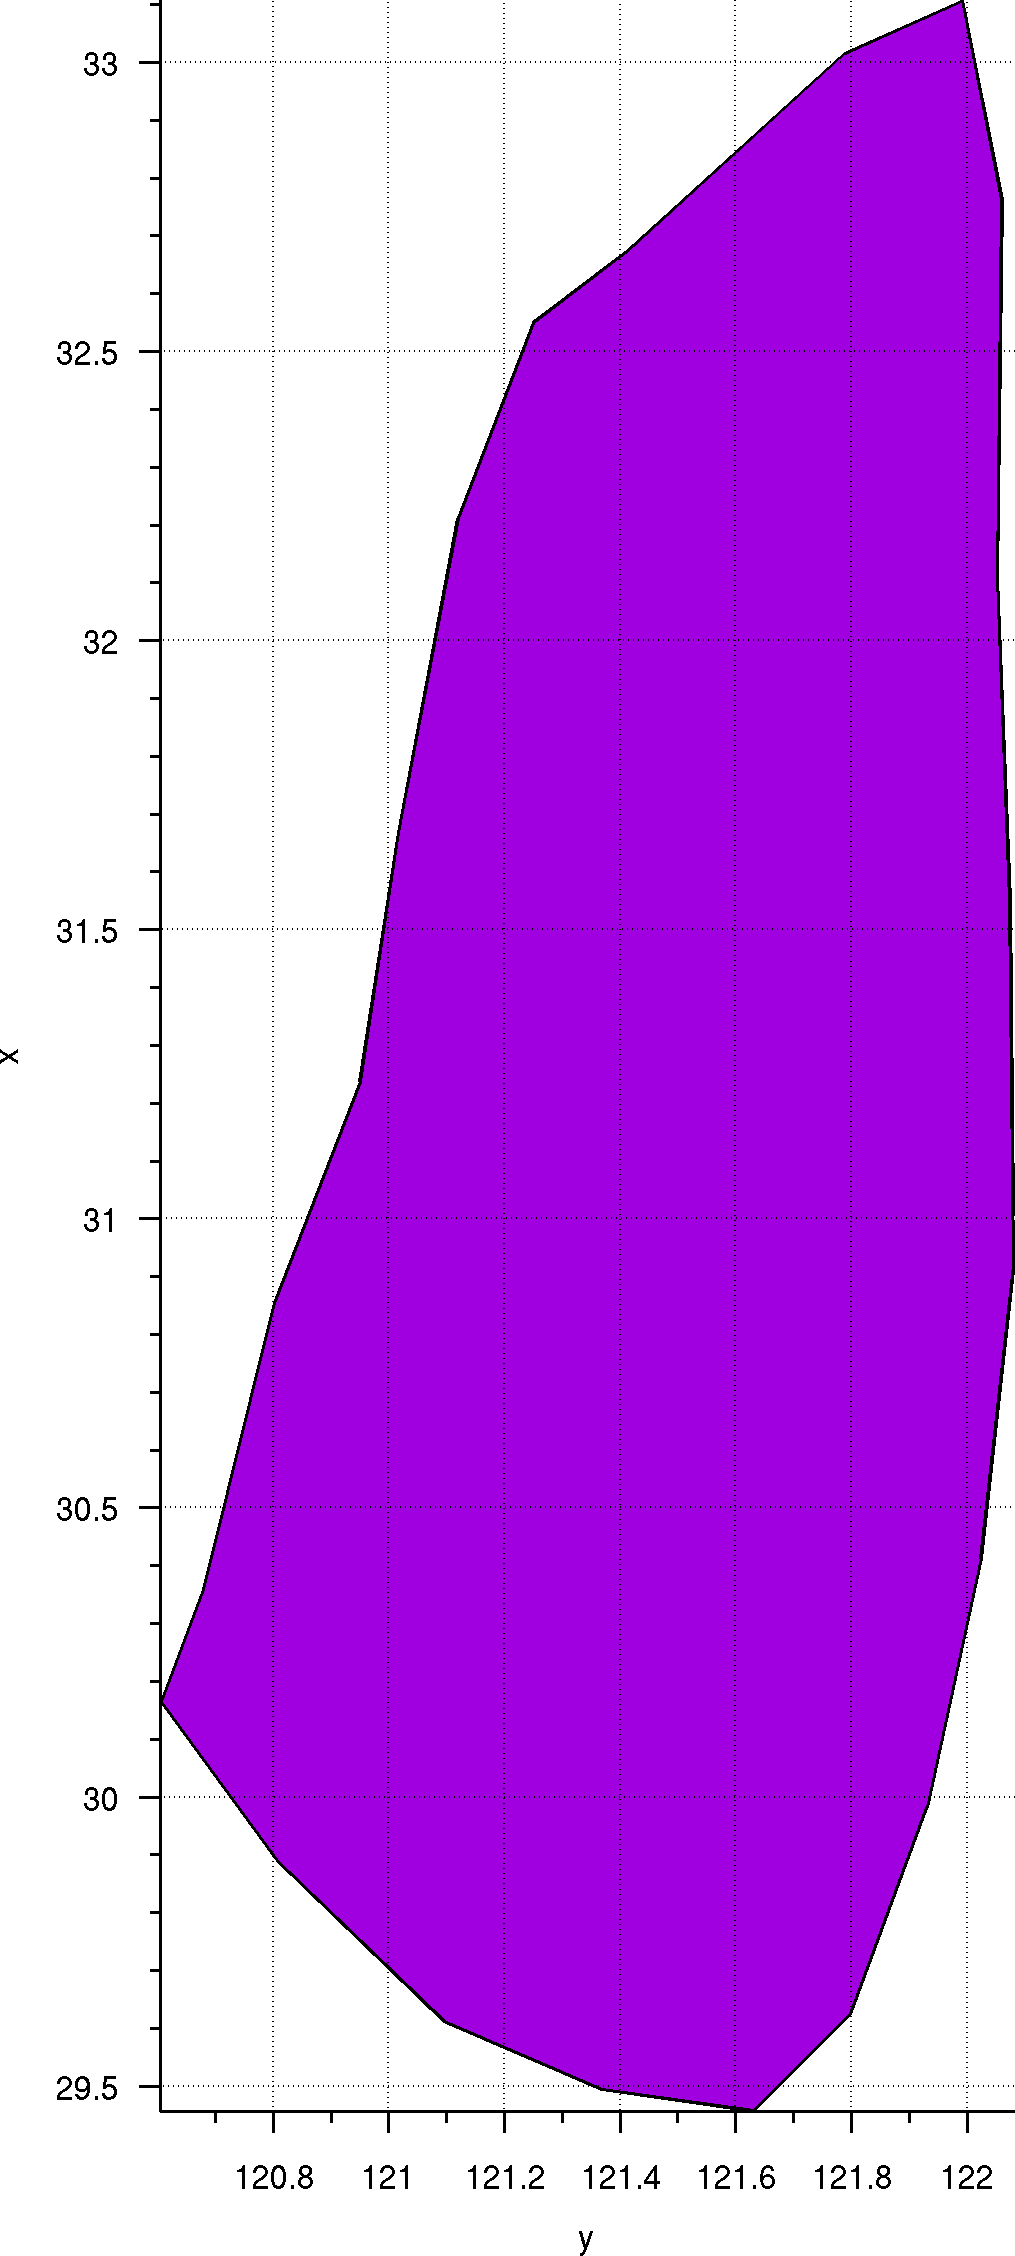
\includegraphics[height=8cm]{pic/grainSmoothed.png}%
      }%
    \end{column}
  \end{columns}

\end{frame}


%

\subsection*{Grain Properties}



\begin{frame}[fragile]
  \frametitle{Grain Properties: Geometry}

Basic functions on grain geometry
\begin{lstlisting}[basicstyle=\footnotesize]
area,perimeter,centroid,hullarea,hullperimeter,
hullcentroid,aspectratio,shapefactor,borderlength,
deltaarea,equivalentperimeter,grainsize,paris
\end{lstlisting}

\begin{columns}[t]
  \begin{column}[T]{6.5cm}

\medskip

  grainsize distribution
\begin{lstlisting}
A = area(grains);
bar( hist(A,exp(-1.5:6.5)) )
\end{lstlisting}

\medskip

other properties:
\begin{lstlisting}[basicstyle=\footnotesize]
hasholes,hassubfraction
\end{lstlisting}

	\end{column}
	\begin{column}[T]{5cm}
		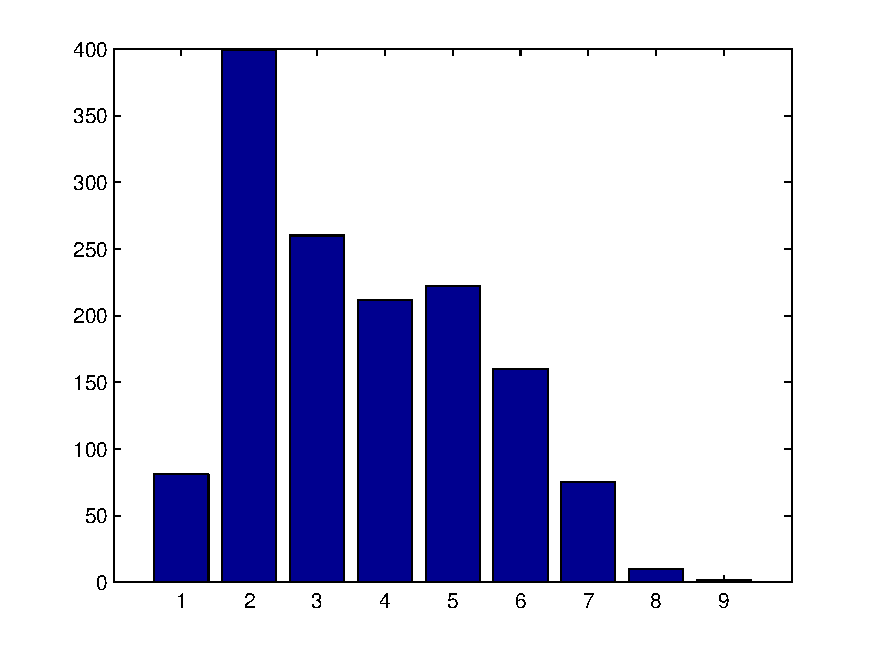
\includegraphics[width=5cm]{pic/grh}
	\end{column}
\end{columns}

select grains by properties
\begin{lstlisting}
grains = grains( area(grains) > mean(area(grains)) )
\end{lstlisting}

\end{frame}


%

\subsection*{EBSD data}


\begin{frame}[fragile]
  \frametitle{Working with EBSD Data Directly}

	Access EBSD Properties
\begin{lstlisting}
	orientations = get(ebsd,'orientation')
	x = get(ebsd,'x')
\end{lstlisting}

	\medskip

	Rotate EBSD Data
\begin{lstlisting}
rot =  rotation('axis',xvector,'angle',90*degree)
ebsd = rotate(ebsd,rot)
\end{lstlisting}

	\medskip
        Omit one pixel grains
\begin{lstlisting}
%grains containing more than one pixel
grains = grains(grainsize(grains) > 1)

%restrict ebsd data to those grains
ebsd = link(ebsd,grains)
\end{lstlisting}

\end{frame}

\subsection*{EBSD - to - ODF Reconstruction}


\begin{frame}[fragile]
  \frametitle{EBSD to ODF Reconstruction in \MTEX}

  \mtex uses kernel density estimation to compute an ODF from EBSD data. The
  sensitive parameter of this method is the kernel function.

\medskip

  Syntax:
  \begin{alertenv}
\begin{lstlisting}
odf = calcODF(ebsd,<options>)
\end{lstlisting}
  \end{alertenv}

Options:
\lstset{emph={bandwidth},emphstyle={}}
\begin{lstlisting}
'kernel'     % the kernel to be used
'halfwidth'  % halfwidth of the kernel function
'resolution' % resolution of the approximation grid

'Fourier'    % ODF by its Fourier coefficients
'exact'      % no approximation to a corser grid
\end{lstlisting}


\end{frame}

\subsection*{Missorientation}

\begin{frame}[fragile]
  \frametitle{Misorientation}

%To treat Misorientation of every grain requires an assigned orientation
%\begin{lstlisting}
%grains = mean(grains,ebsd)
%\end{lstlisting}

Misorientation based on EBSD Data to its mean

\begin{onlyenv}<1| handout:1>
\begin{lstlisting}
/+ebsd_mis = misorientation(grains,ebsd)+/
\end{lstlisting}
\end{onlyenv}
\begin{onlyenv}<2| handout:0>
\begin{lstlisting}
ebsd_mis = misorientation(grains,ebsd)
\end{lstlisting}
\end{onlyenv}

\begin{uncoverenv}<2->
\medskip
Misorientation to neighboured grains
\begin{onlyenv}<1| handout:1>
\begin{lstlisting}
ebsd_mis = misorientation(grains)
\end{lstlisting}
\end{onlyenv}
\begin{onlyenv}<2| handout:0>
\begin{lstlisting}
/+ebsd_mis = misorientation(grains)+/
\end{lstlisting}
\end{onlyenv}

\end{uncoverenv}

%\medskip
\begin{columns}[t]
\begin{column}[T]{6.25cm}
\medskip
Misorientation Distribution
\begin{lstlisting}
hist(ebsd_mis)
\end{lstlisting}

and density function
\begin{lstlisting}
odf = calcODF(ebsd_mis,...)
\end{lstlisting}

\end{column}
  \begin{column}[T]{5.25cm}
\only<1|handout:1>{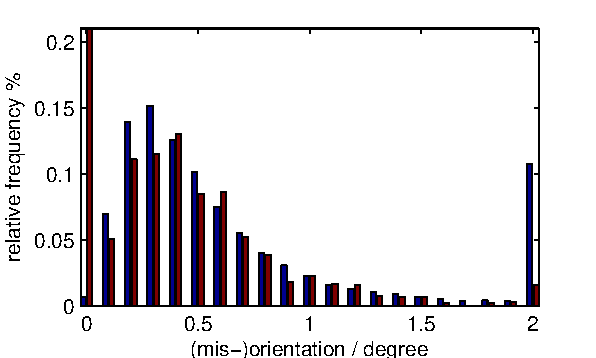
\includegraphics[height=3.5cm]{pic/mis}}
\only<2|handout:0>{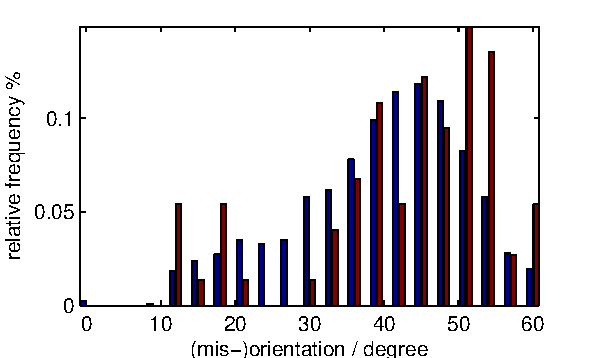
\includegraphics[height=3.5cm]{pic/mis2}}
\end{column}
\end{columns}

\end{frame}


\subsection*{EBSD3d}

\begin{frame}[fragile]
  \frametitle{3D EBSD Data}


\begin{lstlisting}
plot(ebsd)
\end{lstlisting}

\center{
\only<1|handout:1>{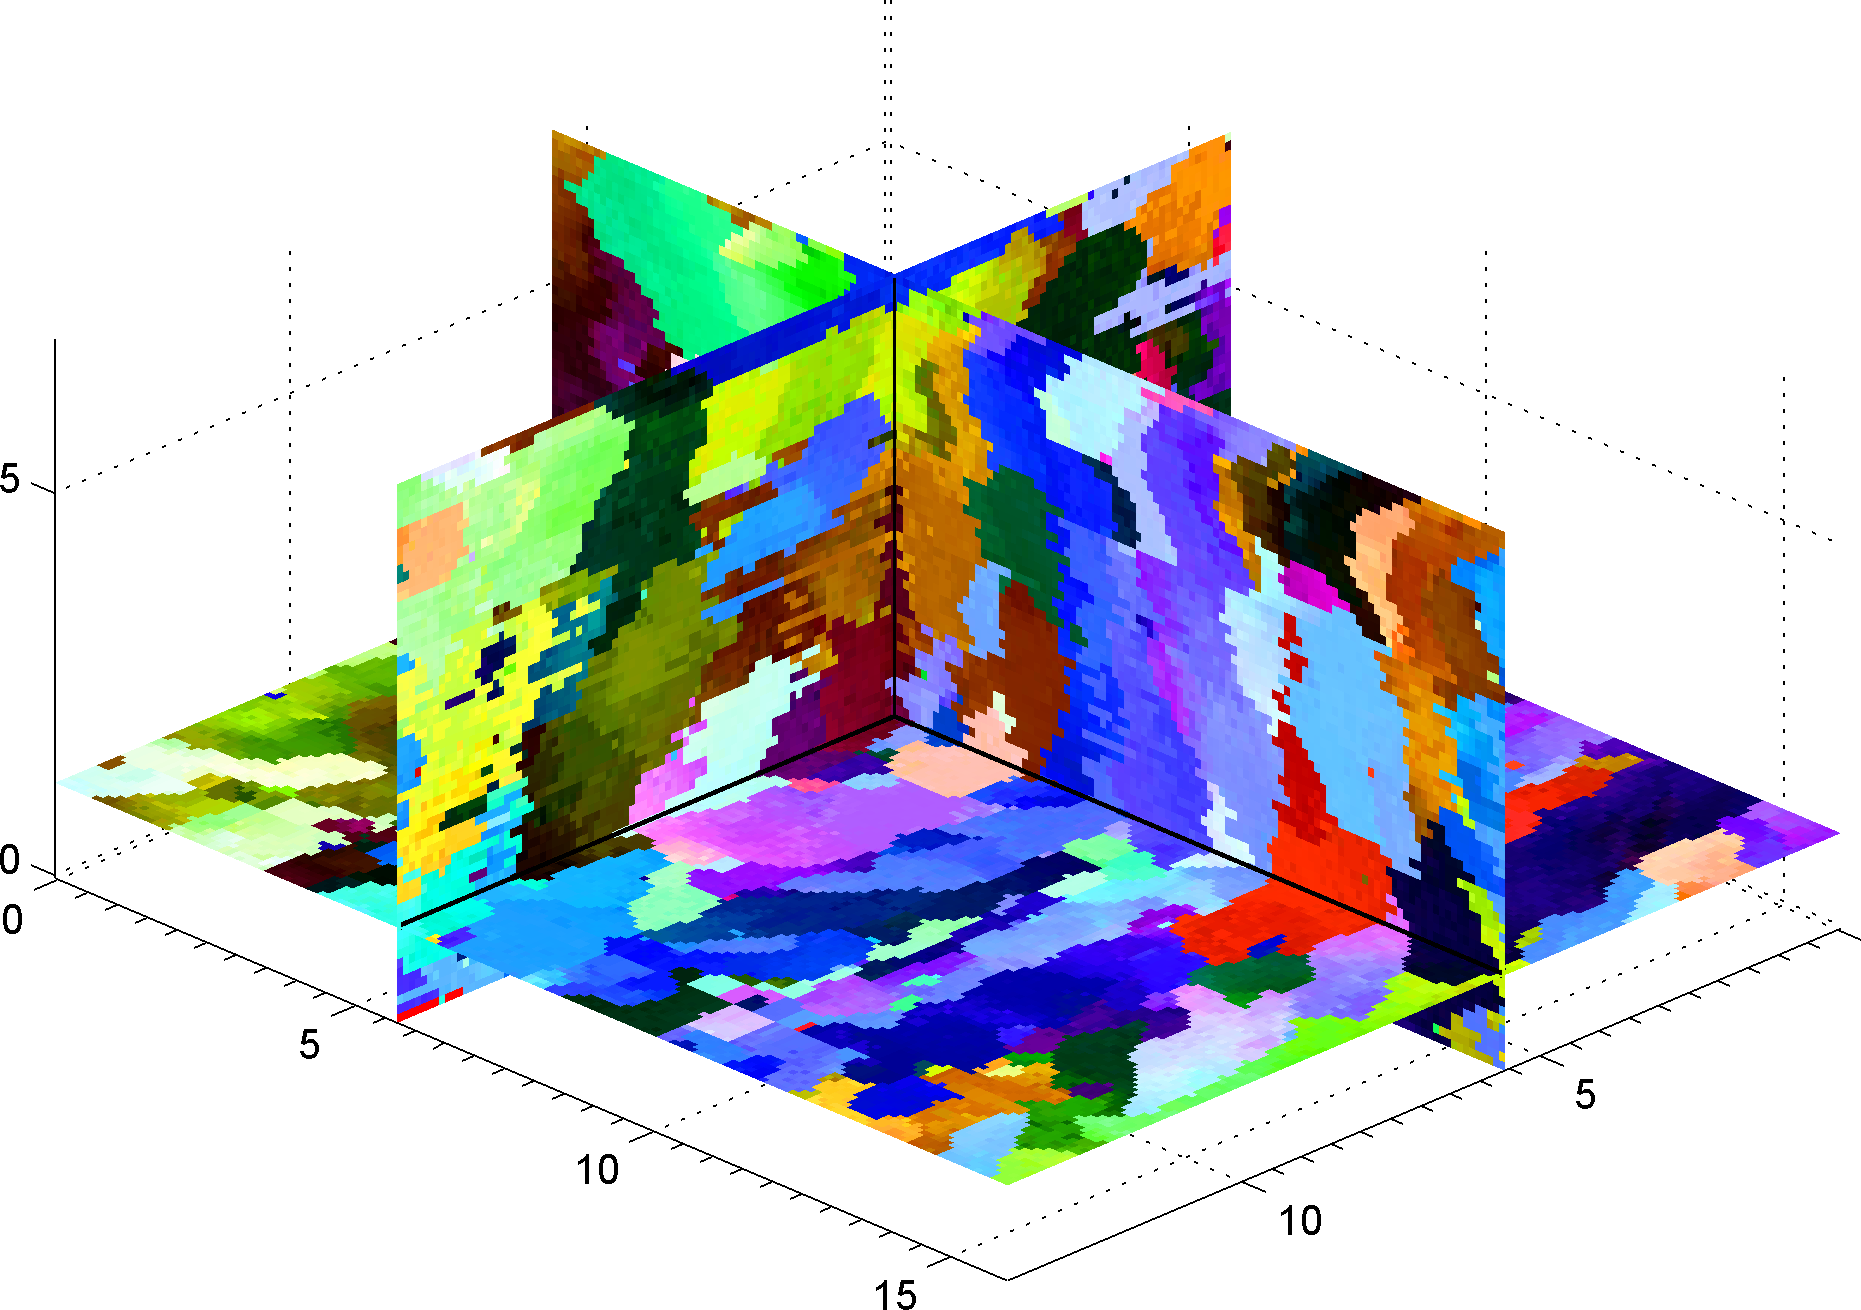
\includegraphics[height=7cm]{pic/3d_slice}}
\only<2|handout:1>{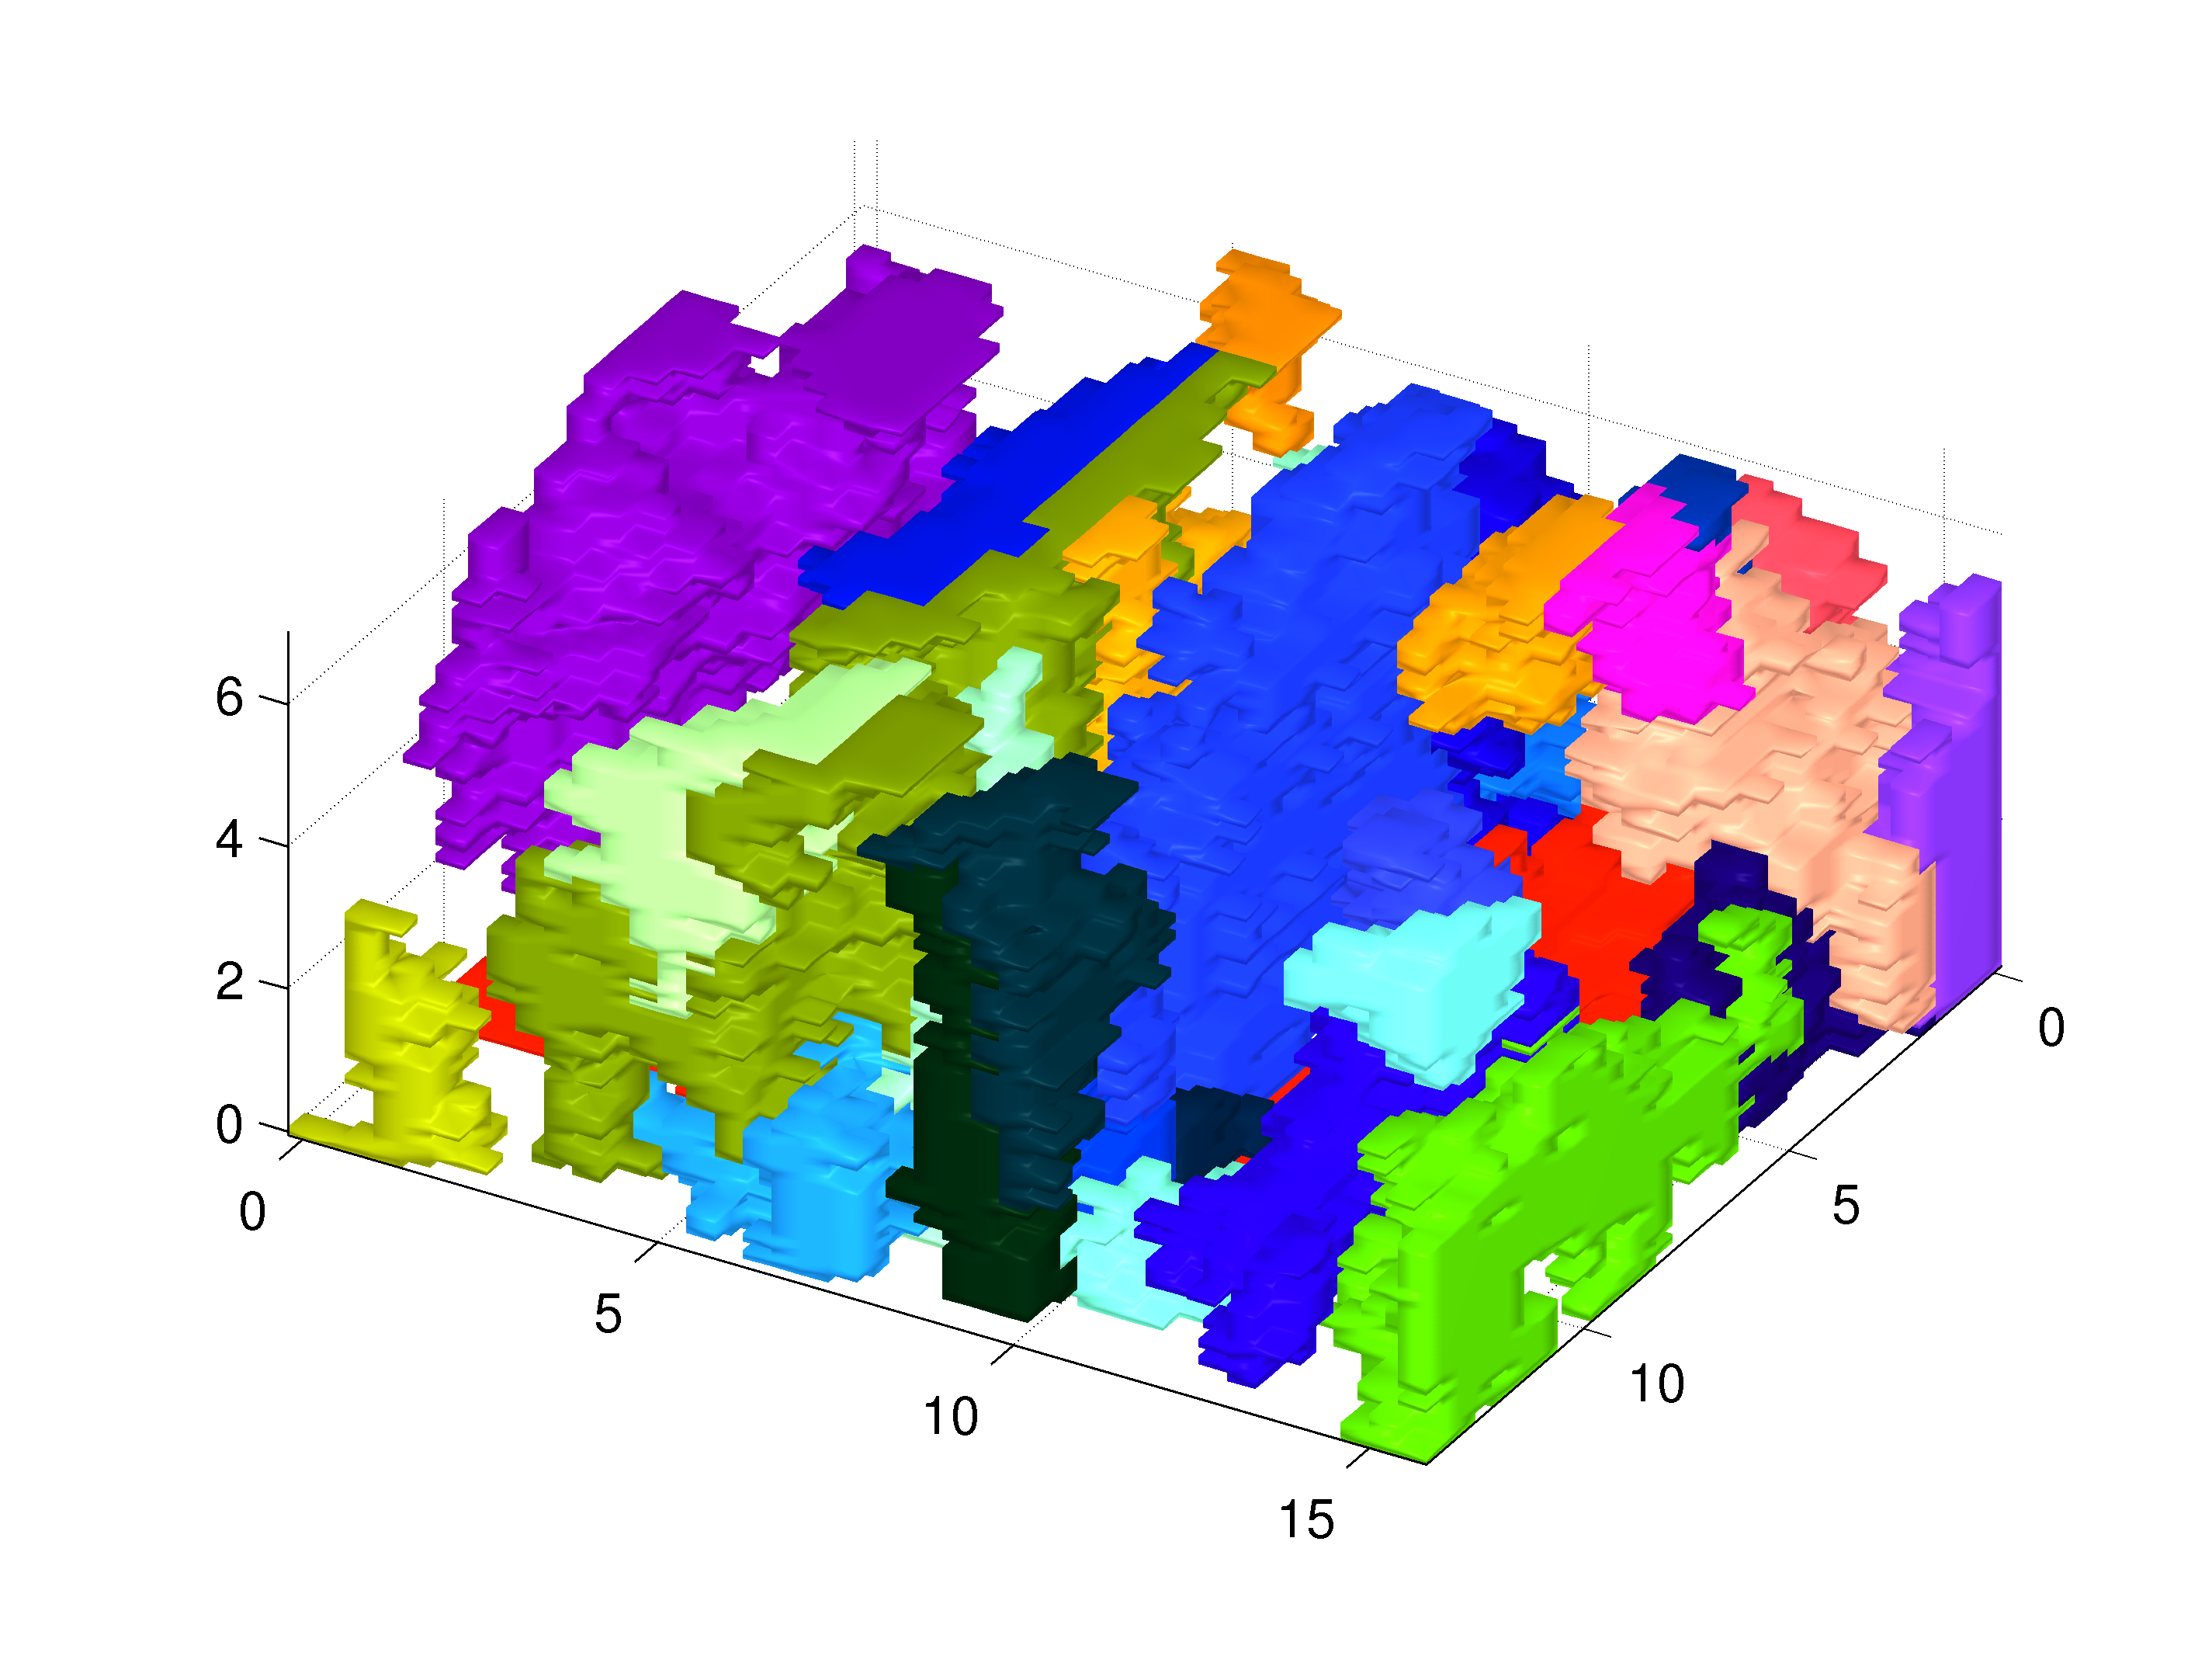
\includegraphics[height=7cm]{pic/3dgrains}}
}

\end{frame}



\subsection*{Exercises}

\begin{frame}

  \begin{Exercise}
    \begin{enumerate}[a)]
    \item Load the EBSD data:
      \texttt{data/ebsd\_txt/85\_829grad\_07\_09\_06.txt}!
    \item Perform grain modelling with a certain threshold!
    \item Plot the EBSD data together with the grain boundaries!
    \item Compute the mean orientation for each grain and visualize it!
    \item Compute and visualize the grain size distribution!
    \item Explore the geometric properties of the grains! Is there any
      relationship between the size and the mad of the grains?
    \end{enumerate}
  \end{Exercise}

  \begin{Exercise}
    \begin{enumerate}[a)]
    \item Estimate an ODF from the above EBSD data.
    \item Visualize the ODF and some of its pole figures!
    \item Explore the influence of the halfwidth on the kernel
      density estimation by looking at the pole figures!
    \end{enumerate}
  \end{Exercise}


\end{frame}

%\begin{frame}

  % \begin{block}{Exercises 6}
  %   \begin{enumerate}
  %   \item Start with an arbitrary model ODF!
  %   \item Compute the volume portion of the ODF within a range of $20\degree$
  %     of the modalorientation and compare it to the corresponding volume of
  %     the uniform ODF!
  %   \item Simulate EBSD data from this ODF with 10.000 orientations.
  %   \item Plot pole figures from the EBSD data and compare them with the pole
  %     figures from the model ODF.
  %   \item Compute the volume portion of the estimated ODF within a range of
  %     $20\degree$ of the modalorientation and compare it to model ODF!
  %   \item Perform these investigations for different sample sizes!
  %   \end{enumerate}
  % \end{block}


%   \begin{Exercise}
%     \begin{enumerate}[a)]
%     \item Estimate an overall grain-ODF and compare it with the ODF of
%       original EBSD data
%     \item Visualize the textureindex of each grain
%     \item Compare the intrinsic misorientation of individual grains to its
%       texture properties, how does the threshold angle affect this?
%     \item Investigate the misorientation of neighbours, how does the threshold
%       angle influence it?
%     \end{enumerate}
%   \end{Exercise}

%\end{frame}



%%% Local Variables:
%%% mode: latex
%%% TeX-master: "main"
%%% End:
